\chapter{Trusted Execution Environment in Blockchain}
Una TEE è un ambiente di protezione che viene utilizzato in diversi contesti, tra cui la blockchain, per permettere l'esecuzione sicura del codice senza correre il rischio di attacchi esterni. Il Trusted Computing ha lo scopo di garantire la sicurezza mediante la realizzazione di una sorta di cassaforte virtuale attorno ai dati ed ai programmi. Se dati o programmi esterni vogliono avere accesso a questa cassaforte devono ottenere la chiave dal sistema di TC e solamente dati e programmi autenticati possono disporre delle risorse del sistema: dall'hard disk, alla memoria RAM, alla CPU. Questo ambiente va a complementare quelle che sono le classiche misure di sicurezza, ovvero protezione di dispositivi, cifratura di informazioni e sviluppo di codice in sicurezza: questo tipo di sicurezza si basa sulla \textit{root of trust}, ovvero la capacità degli endpoint di poter proteggere i dati e le informazioni al loro interno. Questi scenari di sicurezza sono particolarmente indicati per servizi IoT, dove i dispositivi sono facilmente accessibili e quindi devono proteggere le chiavi e i dati presenti al loro interno.

\vspace{5mm}

Per applicare il TC alle applicazioni vengono utilizzate diverse tecniche, tra cui la \textbf{Software Fault Isolation} (SFI), la quale è una tecnica di strumentazione software a livello di codice macchina per stabilire domini di protezione logica all'interno di un processo. Designa una regione di memoria per un componente non attendibile e se in questa sezione si tenta di eseguire accessi alla memoria o a componenti critiche, si vanno a sollevare delle eccezioni. Lavora come sandbox del codice che monitora gli accessi alla memoria.

\section{Esecuzione isolata}
Isolare l'esecuzione del codice è uno degli approcci fondamentali per ottenere la sicurezza. La virtualizzazione può creare un ambiente di esecuzione isolato per l'esecuzione di strumenti difensivi, in quanto molto spesso due programmi che girano su macchine virtuali diverse non possono comunicare, o comunque è possibile monitorare facilmente le comunicazioni: infatti la virtualizzazione per definizione fornisce un ambiente di esecuzione isolato. Gli approcci esistenti basati sulla virtualizzazione hanno limitazioni, tra cui:
\begin{itemize}
    \item dipendenza da hypervisor: gli hypervisor, dato che si occupano di gestire, monitorare, attivare, migrare le macchine virtuali, rappresentano una vera e propria \textbf{Trusted Computing Base} (TCB). Una TCB di un sistema informatico è l'insieme di tutti i componenti hardware, firmware e/o software critici per la sua sicurezza: bug o vulnerabilità che si verificano all'interno del TCB potrebbero compromettere le proprietà di sicurezza dell'intero sistema. In un sistema è desiderabile avere un'ampia base di funzioni scarsamente critiche e una piccola base di funzioni che richiedono protezione. La TCB rappresenta tutto ciò che se dovesse essere attaccato comprometterebbe l'intero sistema, per cui dovrebbe essere più piccola possibile. Nella virtualizzazione l'hypervisor rappresenta la TCB, ma rappresentando un insieme di funzioni molto ampio, non garantisce una sicurezza di base elevata.
    \item mancata gestione dell'hypervisor o dei rootkit del firmware. Un rootkit è una raccolta di software, in genere dannoso, progettato per consentire l'accesso a un computer o a un'area del suo software che non è altrimenti consentito. Un rootkit approfitta di problemi di confidenzialità e integrità dei dati per portare a termine un attacco. L'\textit{availability} può essere vista sotto diversi aspetti: l'availability è vista come disponibilità del sistema, ovvero la capacità del sistema di rispondere a delle richieste. Da un punto di vista di \textit{dependability}, Il sistema potrebbe non rispondere perché si è verificato un fallimento non intenzionale. Nel caso della sicurezza, il fallimento è intenzionale e molto spesso è dovuto proprio ad un attacco mirato. Ovviamente i due fallimenti si gestiscono in modo diverso.
    \item soffre di sovraccarico delle prestazioni del sistema (ad esempio cambi di contesto da una VM a un hypervisor). Questo perché mentre la macchina fisica è unica, possono esserci più macchine virtuali in esecuzione. 
\end{itemize}

Un approccio diverso si realizza con soluzioni container-based, come Docker. Mentre una macchina virtuale astrae l'hardware, i container limitano il loro livello di astrazione al solo sistema operativo con la condivisione dello stesso, con il kernel, la connessione di rete e i file di base. Le istanze vengono eseguite in uno spazio separato, garantendo una diminuzione di consumo della CPU e dell'overload associato. Inoltre i container hanno tempi di arresto e di avvio inferiori ai 50 ms, a differenza delle macchine virtuali che si aggirano nell'ordine di grandezza dei secondi.

\begin{figure}[htb!]
    \centering
    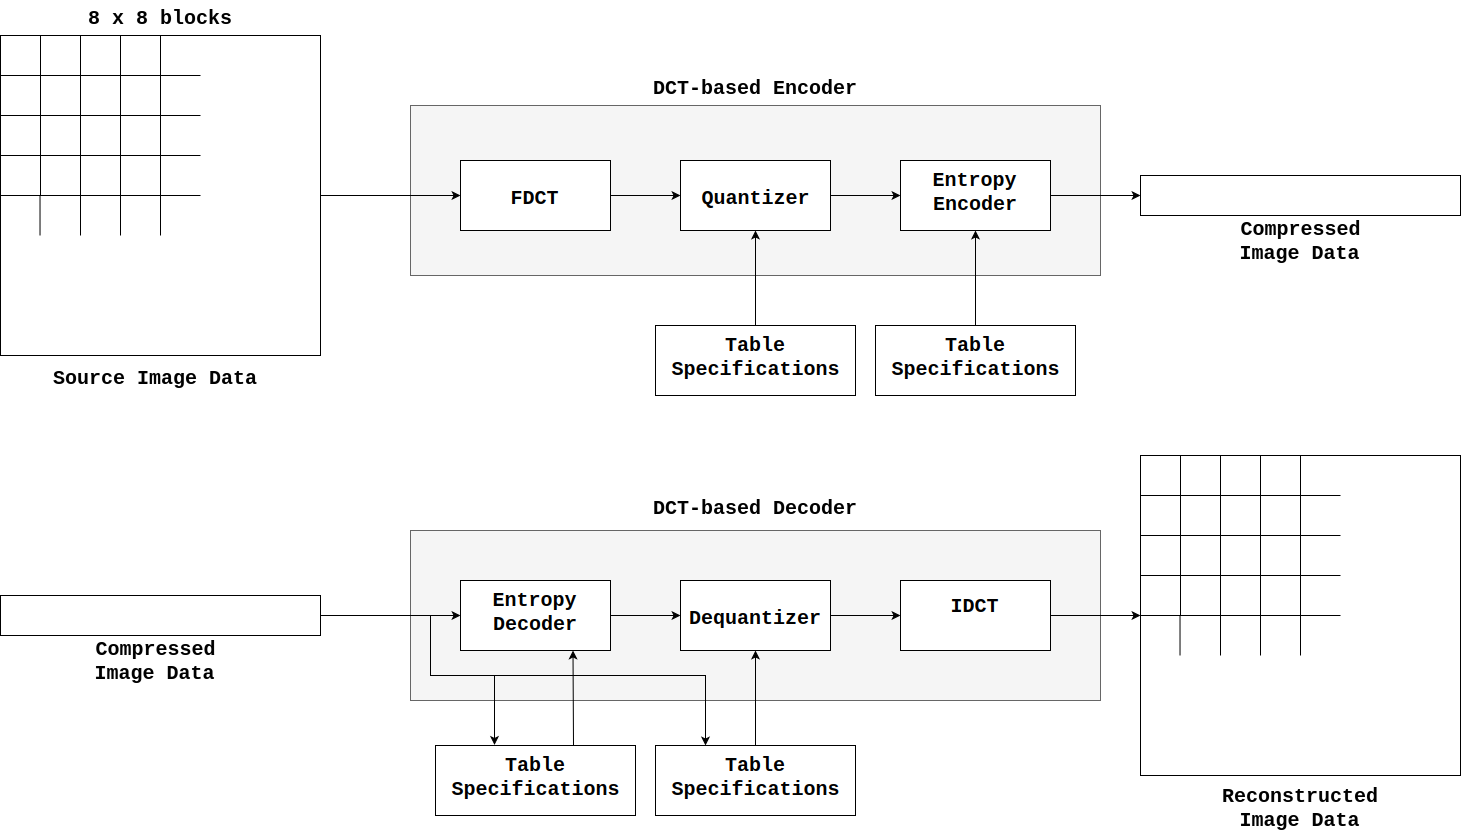
\includegraphics[width=11cm]{./Images/cap6/6.1.png}
\end{figure}

Questa forma di virtualizzazione si basa sui daemon anziché un hypervisor, servizi che sono continuamente in esecuzione, per gestire i container e le immagini delle applicazioni. Gli attacchi per compromettere gli ambienti di esecuzione sono tipicamente basati su vulnerabilità di questi daemon che presentano bug software o cattiva configurazione. Il livello di sicurezza dipende dalla qualità del deamon. Alcune possibilità sono:
\begin{itemize}
    \item Deployment di immagini in container con codice dannoso: le immmagini dannose vengono prima inviate a un registro pubblico per essere estratte e distribuite sugli host Docker non protetti.
    \item Deployment di immagini benigne che scaricano payload dannosi in fase di esecuzione: le immagini benigne vengono distribuite sugli host Docker, dove i payload dannosi vengono quindi scaricati ed eseguiti.
    \item Deployment di file dannosi sulla macchina host: gli avversari montano l'intero file system dell'host su un container e vi accedono dal container. 
    \item Ottenere informazioni sensibili dal registro Docker: gli avversari analizzano i registri Docker per trovare informazioni sensibili.
\end{itemize}
Gli ambienti di esecuzione isolati assistiti da hardware sono stati
realizzati per la protezione dei sistemi, e combinano il concetto
di esecuzione isolata con tecnologie assistite da hardware.
Entrambi sono fondamentali per proteggere i sistemi informatici:
\begin{itemize}
    \item Il concetto di esecuzione isolata fornisce un TEE (Trusted
    Execution Environment) per l'esecuzione di strumenti
    difensivi su un sistema compromesso.
    \item L'utilizzo di tecnologie assistite da hardware esclude gli
    hypervisor dal TCB, raggiunge un alto livello di privilegio
    (ovvero privilegio a livello hardware) e riduce il sovraccarico
    delle prestazioni, consentendo ai cambi di contesto di essere
    eseguiti più velocemente nell'hardware.
    Separa le applicazioni in
    contesti normali e sicuri,
    dove nel secondo è eseguito
    il software critico.
\end{itemize}
\section{Ambienti di esecuzione sicura}
Un ambiente sicuro consente l'archiviazione e l'esecuzione sicure delle
applicazioni.
\begin{itemize}
    \item \textbf{Esecuzione isolata}: ogni applicazione dovrebbe essere eseguita
indipendentemente dalle altre applicazioni.
Un'applicazione dannosa non può accedere ai dati sensibili
conservati da altre applicazioni protette nella memoria.
L'applicazione dannosa non può accedere al codice o ai dati di
un'applicazione mentre è in esecuzione e inoltre non può
alterarne l'esecuzione.
    \item \textbf{Archiviazione sicura}: sono garantite l'integrità e la segretezza di tutti
i dati, inclusi i file binari che rappresentano le applicazioni da
eseguire. i dati più sensibili da proteggere risultano essere le
password, le chiavi di crittografia e i certificati.
    \item \textbf{Provisioning sicuro}: questa proprietà garantisce sia la capacità di
inviare in modo sicuro i dati a un software specifico nell'ambiente
protetto sia la capacità di installare in remoto applicazioni sensibili e
trasferire chiavi di crittografia o certificati.
\end{itemize}
Un'applicazione eseguita in un ambiente che garantisce queste tre
caratteristiche è chiamata applicazione sicura. Le soluzioni di sicurezza hardware hanno il vantaggio di ridurre
notevolmente le intrusioni e gli attacchi.
Gli avversari dannosi possono eseguire attacchi
in grado di ispezionare la memoria di archiviazione o intercettare la chiave durante il
processo di esecuzione, rendendo la crittografia non completamente in grado di affrontare i problemi di sicurezza nel mondo IoT.
La massiccia implementazione della
scheda SIM che incorpora un Secure
Element, ad esempio, è l'origine delle soluzioni
basate su hardware.

Un \textbf{Secure Element} (SE) è un chip a microprocessore in grado di
memorizzare dati sensibili ed eseguire app sicure come i
pagamenti. Agisce come un vault, proteggendo ciò che è
all'interno dell'SE (applicazioni e dati) dagli attacchi malware
tipici dell'host (ovvero il sistema operativo del dispositivo).
Solo le applicazioni firmate dal
produttore possono essere eseguite
in un SE, il che limita le possibilità di
un utente malintenzionato di app e di
un root attacker. Questa è una grande
limitazione per gli sviluppatori e il
motivo principale che ha ostacolato lo
sviluppo di questa tecnologia.

\begin{figure}[htb!]
    \centering
    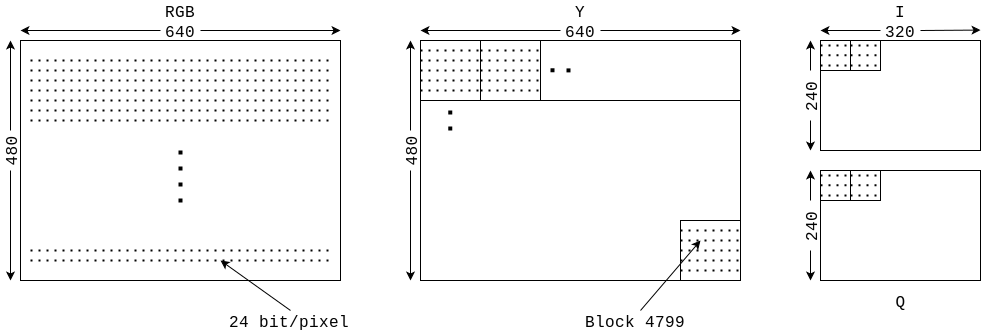
\includegraphics[width=4cm]{./Images/cap6/6.2.png}
\end{figure}
 
Un \textbf{Encrypted Execution Environment} (E3) è un ambiente di
esecuzione in cui il software è crittografato e consente l'esecuzione
senza rivelare le istruzioni che compongono l'applicazione.
È probabile che venga impiegata una società che assegna una
grande quantità di valore monetario e tempo per proteggere i
propri investimenti dalla contraffazione e da altre duplicazioni non
autorizzate.
Ciò non implica necessariamente
che le istruzioni possano essere
eseguite direttamente dal loro
stato crittografato. In effetti, è
accettabile che l'E3 decifri ed
esegua le istruzioni fintanto che
le istruzioni in testo normale non
vengono rivelate esternamente.
Se ogni dispositivo fornito con il
software ha la propria chiave E3, il
software E3 per un dispositivo non
verrà eseguito su un altro.

\begin{figure}[htb!]
    \centering
    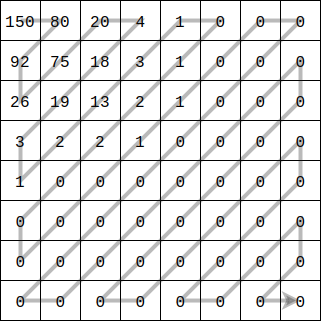
\includegraphics[width=8cm]{./Images/cap6/6.3.png}
\end{figure}

\section{Trusted Platform Module}
Il TPM è costituito da un microcontrollore con funzionalità
crittografiche aggiuntive. Il TPM può essere associato al
dispositivo utilizzando un bus LPC (Low Pin Count) e può
eseguire operazioni crittografiche molto complesse dalla
crittografia simmetrica alla crittografia asimmetrica RSA.
Il vantaggio dell'utilizzo di un TPM è che lo sviluppatore non deve
sapere nulla sull'implementazione di questi algoritmi, poiché il
TPM fornisce un'API (Application Programming Interface).

\begin{figure}[htb!]
    \centering
    \includegraphics[width=8cm]{./Images/cap6/6.4.png}
\end{figure}

Le funzionalità crittografiche di un TPM sono le seguenti:
\begin{itemize}
    \item Acceleratore RSA: un modulo motore esegue le operazioni
crittografiche RSA con una lunghezza massima della chiave
di 2048 bit, ed è utilizzato durante le operazioni di firma
digitale e wrapping delle chiavi.
    \item Il TPM è in grado di calcolare valori hash di piccole porzioni
di dati, come chiavi crittografiche e certificati, ma non è
sufficiente per grandi quantità di dati.
    \item Generazione di numeri pseudo casuali: questa funzione è
molto importante e utile per generare chiavi di crittografia,
ad esempio per RSA.
\end{itemize}
Il TPM è caratterizzato dalla chiave di endorsement, creata
casualmente sul chip al momento della produzione, non può
essere modificata e non lascia mai il chip, mentre la chiave
pubblica viene utilizzata per l'attestazione e per la crittografia dei
dati sensibili inviati al chip.

Le chiavi di identità dell'attestazione vengono conservate dal
TPM per eseguire un'autenticazione con un provider di servizi.
Il TPM archivia tre tipi di certificati:
\begin{itemize}
    \item Il certificato di verifica dell'autenticità garantisce l'integrità
della chiave di verifica dell'autenticità. Questo certificato può
essere fornito dallo stesso emittente dell'EK ma non è
obbligatorio.
    \item Il certificato della piattaforma viene fornito dal fornitore
della piattaforma e garantisce che tutti i componenti di
sicurezza forniti con la piattaforma siano autentici. Questo
certificato abilita l'attendibilità della piattaforma.
    \item Il certificato di conformità viene fornito da un laboratorio di
valutazione di terze parti o dallo stesso fornitore della
piattaforma. Attesta che le proprietà di sicurezza dichiarate
dal produttore sono autentiche.
\end{itemize}
Il TPM protegge i dati mediante due possibili soluzioni: il \textbf{Memory curtaining} estende le comuni tecniche di protezione
della memoria per fornire un isolamento completo delle aree
sensibili della memoria, anche al sistema operativo, ad
esempio le posizioni contenenti chiavi crittografiche. Il \textbf{Sealed storage} invece protegge le informazioni private legandole alle
informazioni di configurazione della piattaforma. I dati possono essere rilasciati utilizzando una chiave che deriva dallo
stato del sistema, ovvero il software utilizzato e l'hardware su
cui è in esecuzione. Le informazioni possono essere utilizzate
solo con la stessa combinazione di software e hardware.
Come caso d'uso, un TPM può essere utilizzato come PKI che
fornisce le chiavi e i certificati necessari per stabilire
comunicazioni protette e firmare documenti.

\section{Trusted Execution Environment}
TEE combina parti hardware e software e consentono di dividere
il sistema in due ambienti di esecuzione.
Il Rich Execution Environment (REE), è
un sistema operativo tradizionale con
notevolmente la superficie di attacco.
Il TEE rappresenta il sistema operativo
sicuro responsabile dell'esecuzione di
operazioni sensibili. Ha anche la
capacità di proteggere il display e
l'ingresso utilizzando una modalità
sicura dei bus che colle-gano il
processore alle periferiche I/O.
Il TEE divide il processore in due zone con un sistema operativo
sicuro e altri meccanismi per migliorare la sicurezza
dell'elaborazione dei dati sensibili.

L'altra caratteristica essenziale è l'archiviazione sicura, in cui i dati
critici e sensibili sono isolati dai dati dell'utente per migliorarne la
sicurezza. In opposizione all'SE, il TEE fornisce un canale di
comunicazione sicuro tra il processore e la periferica esterna, in
particolare l'ingresso e il display. Se un'applicazione dannosa può intercettare l'input, può avere
accesso a dati sensibili. Anche la visualizzazione sicura è primordiale
perché l'utente deve essere sicuro che ciò che vede sullo schermo
sia realmente inviato dal mondo sicuro.
È inoltre necessario un processo di avvio sicuro:
\begin{enumerate}
    \item Leggere una ROM affidabile (bloccata in produzione).
    \item Controllo della firma e dell'integrità del sistema operativo sicuro.
    \item Configurazione del sistema operativo sicuro.
\end{enumerate}
TEE ha anche una terza modalità chiamata Monitor, utilizzata per
eseguire il salvataggio del contesto e il passaggio tra Rich e Secure OS. Il sistema operativo sicuro ha un set di istruzioni limitato,
necessario per ridurre la superficie di attacco, e pianifica le
applicazioni sensibili in esecuzione su di esso per realizzare
istruzioni sicure come operazioni crittografiche: generazione di
chiavi, crifratura/decifratura di dati, generazione di firme.
SE e il TPM hanno più funzionalità di sicurezza fisica rispetto a
TEE. Tuttavia, TEE fornisce una maggiore potenza di calcolo che
consente modelli di sicurezza più complessi. Nella tabella possiamo vedere le differenze.

\begin{figure}[htb!]
    \centering
    \includegraphics[width=12cm]{./Images/cap6/6.5.png}
\end{figure}

La base per la realizzazione a livello hardware di
TEE è costituita da coprocessore, che sono un
processore specializzato che esegue algoritmi
crittografici a livello hardware e accelera il
processo di cifrature/decifratura per una migliore
sicurezza dei dati e protezione delle chiavi
segrete.
Un processore generico (GPP) viene personalizzato e utilizzato
per implementare alcuni algoritmi crittografici. La personalizzazione principale sono le estensioni del set di istruzioni (possono
essere chiamate istruzioni crittografiche) per applicazioni
crittografiche. In questo caso, le chiavi segrete vengono salvate
nella memoria principale e utilizzate come altri normali dati
. Un coprocessore crittografico è un modulo esterno al
GPP che accelera i calcoli crittografici. Le chiavi segrete
normalmente non vengono memorizzate nella memoria
del coprocessore, ma nei registri dati del processore o
nella memoria principale. Il coprocessore crittografico
può essere controllato utilizzando il GPP host.

Ci sono molti modi in cui questi TEE possono essere realizzati.
\begin{enumerate}
    \item La prima realizzazione utilizza un coprocessore di sicurezza per scaricare le
attività critiche per la sicurezza dall'ambiente operativo principale. I vantaggi sono che l'operazione può essere generalmente
completamente isolata e può essere eseguita simultaneamente con il
nucleo principale. Lo svantaggio è che c'è un sovraccarico associato al trasferimento dei dati
da e verso il core.
Può avere un coprocessore di sicurezza esterno (con HSM) o integrato (TPM). Un TPM è un chip hardware sulla scheda madre ed è in grado di fornire la crittografia completa dei dischi. TPM mantiene i dischi rigidi bloccati fino a quando il sistema non completa una verifica del sistema o un processo di autenticazione. D'altra parte, HSM è un dispositivo removibile o esterno che genera, archivia e gestisce chiavi crittografiche.
    \item Molte famose architetture TEE supportano un nuovo tipo di configurazione in
cui un singolo core supporta più core virtuali che si escludono a vicenda,
ovvero quando uno è in esecuzione l'altro è sospeso. Normalmente questa
transizione da uno stato all'altro viene eseguita da una sorta di monitor/trigger. Questa configurazione viene talvolta definita "ambiente protetto del
processore".
Esempi sono ARM TrustZone e Intel Trusted Execution Technology.
    \item Oltre alle tecniche basate sull'hardware, sono stati presentati altri approcci,
come XOM (eXecute-Only-Memory) a livello di architettura. Tali piattaforme
realizzano il TEE per separazione architettonica, previene la fuoriuscita di
informazioni dalle applicazioni XOM utilizzando il compartimento, dove un
compartimento è un contenitore logico che impedisce alle informazioni di
entrare o uscire da esso.
Ulteriori esempi di software TEE includono i contenitori Docker.
\end{enumerate}

\begin{figure}[htb!]
    \centering
    \includegraphics[width=11cm]{./Images/cap6/6.6.png}
\end{figure}

\subsection{Processori ARM TrustZone}
Il processore ARM TrustZone ha un'istruzione specifica chiamata Secure
Monitor Call (SMC) da invocare durante l’esecuzione nel mondo normale per
entrare in "modalità monitor" che esegue la transizione al mondo sicuro.
\begin{itemize}
    \item Non è necessario scaricare i dati da / verso il mondo sicuro. È previsto un
costo aggiuntivo per memorizzare / ripristinare lo stato del dispositivo
all'ingresso / uscita da una determinata modalità.
    \item Lo svantaggio è che quando un mondo è attivo, l'altro deve essere
completamente fermato, complicando così la gestione delle interruzioni.
\end{itemize}
L'innovazione architettonica più significativa
è l'aggiunta di un nuovo bit del processore, il
33-esimo, che indica in quale modo il
processore è attualmente in esecuzione.
Il TrustZone address space controller (TZASC)
estende la sicurezza a livello di memoria,
abilitando la partizione in differenti regioni.
L'unità di gestione della memoria (MMU) che riconosce la zona di fiducia
fornisce due interfacce MMU distinte.

L'API TrustZone (TZAPI) specifica in che modo le applicazioni non protette
(NSA), in esecuzione nell'ambiente ricco, interagiscono con l'ambiente di
esecuzione isolato.
Seguendo un modello client-server, l'API definisce un insieme di interfacce
software astratte mediante le quali un NSA può interagire con un TA. L'API
consente ai client di inviare comandi e richieste a un TA e scambiare dati tra i
due mondi. L'API TrustZone non include alcuna specifica su come sviluppare
applicazioni in esecuzione all'interno dell'ambiente di esecuzione isolato.

\begin{figure}[htb!]
    \centering
    \includegraphics[width=11cm]{./Images/cap6/6.7.png}
\end{figure}

\subsection{Intel SGX}
Tecniche come Intel Software Guard Extensions (Intel SGX) utilizzano sia
hardware che software per implementare TEE.
Le applicazioni Intel SGX sono costituite
da una parte affidabile e una parte non
attendibile. Quando l'applicazione deve
lavorare con un segreto, crea un'enclave
che viene collocata nella memoria
attendibile. Quindi chiama una funzione
attendibile per entrare nell'enclave,
dove gli viene fornita una visualizzazione
dei suoi segreti in testo chiaro.
Tutti gli altri tentativi di accesso alla memoria dell'enclave dall'esterno
dell'enclave sono negati dal processore, anche quelli effettuati da utenti
privilegiati. Ciò impedisce che i segreti nell'enclave vengano svelati.

SGX è un insieme di istruzioni della CPU che consentono a un'applicazione di
istanziare un contenitore protetto, denominato enclave. Un'enclave è definita come un'area protetta nello spazio degli indirizzi
dell'applicazione che non può essere alterata da codice esterno
all'enclave, nemmeno da codice con privilegi superiori. Il core non esegue una transizione completa, ma parti di un'applicazione
standard sono protette da meccanismi hardware nel core. I vantaggi sono che non è necessario trasferire i dati avanti e indietro tra
i core o impostare transizioni complicate da e verso un mondo sicuro e
non è necessario un ambiente operativo separato come richiesto in altri
stili di configurazione TEE. Il componente affidabile dovrebbe essere il più piccolo possibile: una
grande enclave con un'interfaccia complessa non consuma solo più
memoria protetta: crea anche una superficie di attacco più ampia. Le enclave dovrebbero anche avere un'interazione minima tra
componenti attendibili e non attendibili: limitare queste dipendenze
rafforzerà l'enclave contro gli attacchi.

\textbf{Untrusted Run-Time System} (uRTS) indica
il codice che viene eseguito al di fuori
dell'ambiente enclave ed esegue il
caricamento e la manipolazione di
un'enclave, l'esecuzione di chiamate
(ECALL) a un'enclave e la ricezione di
chiamate (OCALL) da un'enclave.
\textbf{Trusted Run-Time System} (tRTS)
rappresenta il codice che viene
eseguito all'interno dell'ambiente
dell'enclave ed esegue la ricezione
di chiamate (ECALL) dall'applicazione e l'esecuzione di chiamate
all'esterno (OCALL) dell'enclave o la
gestione dell'enclave stessa.

\begin{figure}[htb!]
    \centering
    \includegraphics[width=13cm]{./Images/cap6/6.8.png}
\end{figure}

\subsection{Open TEE}
Agli sviluppatori di applicazioni mancano le interfacce per utilizzare le
funzionalità TEE basate su hardware. In effetti, il loro utilizzo è stato limitato
principalmente alle applicazioni sviluppate dai fornitori di dispositivi. La
recente standardizzazione delle interfacce TEE da parte di Global Platform
(GP) promette di risolvere parzialmente questo problema consentendo alle
applicazioni conformi a GP di essere eseguite su TEE di diversi fornitori.
Gli sviluppatori ordinari che desiderano sviluppare applicazioni affidabili
devono affrontare sfide significative. È difficile ottenere l'accesso alle
interfacce hardware TEE senza alcun supporto da parte dei fornitori. Gli
strumenti e il software necessari per sviluppare ed eseguire il debug di
applicazioni affidabili possono essere costosi o inesistenti, con solo tecniche
di debug primitive come il "tracciamento di stampa".
Un TEE virtuale chiamato Open-TEE, conforme alle specifiche GP, è stato
proposto come TEE virtuale conforme agli standard implementato
interamente nel software consentirà agli sviluppatori di creare applicazioni
TEE utilizzando strumenti e ambienti di sviluppo con cui hanno già familiarità.

La specifica GP è composta da:
\begin{itemize}
    \item L'API TEE Core, che fornisce un ampio set
di funzionalità, come un'API crittografica e uno storage sicuro, per
implementare un TA.
    \item L'API client TEE: è uno strato molto
generico e sottile costituito da un
numero limitato di funzioni e
definizioni per trasferire i dati avanti
e indietro da REE a TA.
\end{itemize}
Tra l'API client TEE in esecuzione su REE e l'API TEE Core in esecuzione su TEE,
abbiamo un'efficace RPC (Remote Procedure Call) in cui un processo in
esecuzione in REE può richiamare attività nel TEE.
Questi sforzi di standardizzazione nella piattaforma globale potrebbero
risolvere il problema dei TEE interoperabili. Tuttavia, non rimuovono
l'ostacolo all'accesso all'hardware richiesto né semplificano il compito di
sviluppare e testare le TA.

\begin{figure}[htb!]
    \centering
    \includegraphics[width=12cm]{./Images/cap6/6.9.png}
\end{figure}

Open-TEE fornisce un'architettura e un kit di sviluppo software (SDK) che
implementa le specifiche GP come framework e un insieme di strumenti
familiari allo sviluppatore, eliminando così la necessità di hardware
specializzato e le spese generali che comporta.
\begin{itemize}
    \item Open-TEE è progettato per funzionare
come un processo demone nello
spazio utente. Inizia l'esecuzione di
Base, un processo che incapsula la
funzionalità TEE nel suo complesso.
Una volta inizializzato, Base eseguirà il
fork per creare due processi indipendenti ma correlati.
    \item Manager può essere visualizzato come il
"sistema operativo" di Open-TEE: si occupa della gestione delle connessioni tra le
applicazioni, del monitoraggio dello stato del TA, di fornire archiviazione sicura per TA e del controllo delle regioni di memoria
condivisa per le applicazioni.
La centralizzazione in un processo di
controllo può anche essere visto come
un wrapper che astrae l'ambiente in
esecuzione e lo riconcilia con i requisiti
imposti dagli standard GP TEE.
    \item L'unico scopo di Launcher è creare
nuovi processi TA in modo efficiente.
Quando viene creato per la prima
volta, Launcher caricherà una libreria
condivisa che implementa l'API TEE
Core e attenderà ulteriori comandi da
Manager. Manager segnalerà Launcher quando
è necessario avviare un nuovo TA.
    \item Dopo aver ricevuto il segnale,
Launcher si clonerà da solo. Il clone
caricherà quindi la libreria condivisa
corrispondente al TA richiesto.
\item Il design di Launcher segue il modello
di progettazione "zigote".
Zygote è un processo speciale del
sistema operativo Android che
abilita il codice condiviso su Dalvik/Art VM in contrasto con Java VM
in cui ogni istanza ha la propria
copia dei file di classe della libreria
principale e degli oggetti heap.
\item Un processo TA appena creato viene
quindi reimpostato su Manager in
modo che sia possibile controllarlo.
\item I processi TA sono stati divisi in due fili.
Il primo gestisce Inter-Process
Communication (IPC) e il secondo è il
thread di lavoro, indicati rispettivamente come thread IO e TA Logic. Questo modello architettonico
consente di interrompere il processo
senza arrestarlo e consente una
maggiore separazione e astrazione
della funzionalità TA dal framework
Open-TEE.
\item L'API client TEE e l'API TEE Core sono
implementate come librerie condivise
per ridurre il consumo di codice e
memoria. Open-TEE implementa un protocollo
di comunicazione oltre ai socket del
dominio Unix e ai segnali di interelaborazione come mezzo per
controllare il sistema e trasferire i
messaggi tra CA e TA.
\end{itemize}

\section{Applicazione di TEE nelle Blockchain}
Vedremo due applciazioni del Trusted Execution Environment nella blockchain: Hyperledger Sawtooth e Hyperledger Avalon.

\subsection{Hyperledger Sawtooth}
Hyperledger Sawtooth è una piattaforma blockchain aziendale
altamente modulare che consente alle applicazioni di scegliere le
regole di transazione, i permessi e gli algoritmi di consenso che
supportano le loro esigenze aziendali uniche.
Sawtooth semplifica lo sviluppo e la distribuzione di un'applicazione
fornendo una chiara separazione tra il livello dell'applicazione e il livello
del sistema principale.
Sawtooth fornisce un'astrazione
degli smart contracts che
consente agli sviluppatori di
applicazioni di scrivere la logica
del contratto in una lingua a loro
scelta, inclusi Python, Javascript,
Go, C ++, Java e Rust.

\begin{figure}[htb!]
    \centering
    \includegraphics[width=10cm]{./Images/cap6/6.10.png}
\end{figure}

Sawtooth rappresenta lo stato per tutte le famiglie di transazioni in una singola istanza di un
albero Merkle-Radix su ogni validatore, ovvero un Merkle tree indirizzabile dove gli indirizzi
identificano in modo univoco i percorsi ai nodi foglia dell'albero in cui sono archiviate le
informazioni.
Il processo di convalida dei blocchi su ciascun validatore garantisce che le stesse transazioni
risultino nelle stesse transizioni di stato e che i dati risultanti siano gli stessi per tutti i
partecipanti alla rete.

Sawtooth astrae i concetti fondamentali del consenso e isola il
consenso dalla semantica delle transazioni. L'interfaccia di consenso
Sawtooth supporta il collegamento di varie implementazioni di
consenso come consensus engines che interagiscono con il
validatore attraverso l'API di consenso e di comunicazione P2P.
Sawtooth consente di modificare il consenso dopo che la rete è stata
creata ed è in esecuzione con una o due transazioni.

Il consenso Proof of Elapsed Time (PoET)
offre una soluzione al problema dei generali
bizantini che utilizza un "ambiente di esecuzione affidabile" per migliorare l'efficienza
delle soluzioni attuali come Proof-of-Work.
PoET sceglie stocasticamente i peer
per eseguire le richieste, e comportamenti fraudolenti sono evitati
da TEE e verifica di
identità. PoET funziona essenzialmente come segue:
\begin{itemize}
    \item Ogni validatore richiede un tempo di attesa da un'enclave
(mediante l’esecuzione di una funzione attendibile).
    \item Il validatore con il tempo di attesa più breve per un particolare
blocco di transazione viene eletto leader.
    \item Una funzione, come "CreateTimer", crea un timer per un blocco
di transazioni che è garantito essere stato creato dall'enclave.
    \item Un'altra funzione, come "CheckTimer", verifica che il timer sia
stato creato dall'enclave. Se il timer è scaduto, questa funzione
crea un'attestazione che può essere utilizzata per verificare che il
validatore abbia atteso il tempo assegnato prima di rivendicare il
ruolo di leadership.
\end{itemize}
Questo algoritmo rientra nella casistica basati sulla lotteria come
quello di Nakamoto.

In generale, le soluzioni BFT possono resistere a comportamenti
malizioni di alcuni nodi. Le soluzioni CFT presumono che nessun
nodo sia malizioso, ma può bloccarsi o scomparire dalla rete senza
anomalie nel suo comportamento. Le soluzioni CFT sono
generalmente meno costose e qui scalabili. PoET con hardware SGX realizza un consenso BFT: l'enclave SGX
genera in modo sicuro il valore del tempo di attesa casuale a
prova di manomissione. L'enclave firma quindi un certificato con
il valore del tempo di attesa. Dopo la scadenza del timer,
l'attestazione SGX viene inviata agli altri nodi di rete. I nodi peer
verificano la firma del tempo di attesa generata dal nodo
vincente. Il nodo vincente può pubblicare il blocco proposto. PoET è disponibile anche senza SGX, che è simulato. Data tale
simulazione, il consenso sarà solo CFT non BFT.

\subsection{Hyperledger Avalon}

Le blockchain offrono consistenza e trust tramite una replica
massiccia dei dati, ma hanno un throughput limitato e privacy e
riservatezza imperfette.
On-chain sono le transazioni che
consistono in una transizione di stato
con consenso globale.
SideChain è una soluzione di pochi nodi
che mantiene un consenso locale per
determinate informazioni estratte dalla
catena principale.
Off-chain sono elaborazioni su dati
estratti dalla catena.
L’aggiunta di un'esecuzione off-chain affidabile a una blockchain è
proposta come la soluzione per migliorare le prestazioni.

\begin{figure}[htb!]
    \centering
    \includegraphics[width=9cm]{./Images/cap6/6.11.png}
\end{figure}


Una blockchain principale mantiene una singola istanza autorevole
degli oggetti, applica le politiche di esecuzione e garantisce la
verifica delle transazioni e dei risultati, mentre l’elaborazione offchain associato consente una maggiore produttività. Si rende
necessario abinare soluzioni di trusted computing per aumentare
l'integrità delle processazioni e proteggere la riservatezza dei dati.
Ogni azienda ha richiedenti che inviano transazioni e i worker li
eseguono. Le ricevute
sono registrate sulla
blockchain.

\begin{figure}[htb!]
    \centering
    \includegraphics[width=11cm]{./Images/cap6/6.12.png}
\end{figure}

Le richieste di elaborazioni verso workers ospitati in un enclave TEE
sono inviati dai richiedenti tramite l'interfaccia utente front-end o
strumenti a riga di comando. Gli ordini di lavoro possono essere
inviati anche da smart contract in esecuzione su DLT. Esistono due
modelli di funzionamento:
\begin{itemize}
    \item Modello proxy per smart contract con componenti che
implementano le interazioni tra DLT e TCS o
connettori che astraggono le API specifiche di
un DLT o un proxy
Avalon invocabile dai
richiedenti mediante la
sintassi della DLT.
    \item Modello diretto, che fornisce un'API RPC JSON.
\end{itemize}
Può essere utilizzato
anche un modello ibrido
che combina elementi di
entrambi i modelli proxy
e diretti. Tutte le comunicazioni tra i componenti front-end e middleware vengono effettuate tramite
KV Storage Manager, che mantiene una directory dei worker con tutte le informazioni sull'attestazione, sul tipo (singleton o
pool) e i parametri di esecuzione (es. pod K8S, numero massimo consentito di istanze
simultanee), e una coda ordini di lavoro, che contiene richieste di ordini di lavoro, risposte e,
facoltativamente, ricevute
Il KV Storage Manager è un thin wrapper di Lightning Memory-Mapped Database (LMDB) che
rappresenta una libreria software per fornire un database transazionale ad alte prestazioni
sotto forma di archivio di valori-chiave. Il Worker Manager è
responsabile della creazione
della chiave crittografica del
worker mediante Worker Key
Manager (WKM) per i pool di
worker, della creazione e
manutenzione dei pool di
worker. Il gestore della limita il flusso di richieste per un dato
worker, serializza l'esecuzione delle richieste esprimenti
delle dipendenze esplicitamente specificate, secondo il
modello più letture e una scrittura. Avvia l'esecuzione
della richiesta tramite uno o più adattatori di esecuzione
e gestisce la dimensione della coda con la rimozione di
richieste troppo vecchie. 

L’interazione con i worker fondamentalmente avviene
con un'interazione diretta con istanze di worker allocati
singolarmente o come pool, in maniera statica o
dinamica.
In aggiunta è possibile prevedere che i worker siano
impacchettati come pod K8S e vengono avviati tramite
l'API di Kubernetes, così da avere un motore di
coordinamento e loadbalancing tra di essi. Inizialmente un nuovo worker viene istanziato in un enclave con
apposito manager. Le sue informazioni di attestazione vengono
generate e pubblicate sulla blockchain (o/e su un server). Successivamente un richiedente cerca un worker, ne verifica le
informazioni di attestazione e le memorizza per un ulteriore utilizzo. Il richiedente crea una richiesta di lavoro e lo memorizza sulla blockchain. Il manager preleva
l’ordine e lo inoltra a un
worker nell’enclave. A conclusione, la risposta
è posta nella blockchain
e viene reperita dal
richiedente. L'implementazione Avalon esistente fornisce l'attestazione e la
registrazione dei lavoratori, l'applicazione dell'integrità e della
riservatezza degli richieste end-to-end, la loro elaborazione
asincrona, il modello diretto e l'integrazione con le blockchain Fabric
ed Ethereum.
Open Enclave con
supporto SGX è
impiegato per
l’implementazione
dell’enclave dove
eseguire i worker.

\clearpage
\section{Prova di esempio dell'esame}
Ogni esercizio vale 6 punti. Durata della prova 1 ora.

\vspace{5mm}

\subsubsection{\textbf{ESERCIZIO 1} - Descrivere il significato del seguente script BitCoin:}

\begin{center}
    \texttt{2DUP EQUAL NOT VERIFY SHA256 SWAP SHA256 EQUAL}
\end{center}

\textbf{Soluzione:} come sappiamo gli script bitcoin lavorano sul top dello stack, inserito nella chiave che serve per sbloccare la transazione. \texttt{DUP} sta per \textit{duplication}, quindi prendo i primi due elementi dello stack, lo duplico, e li rimetto nello stack. Quindi se nello stack avevo la stringa \texttt{AB}, ora ho \texttt{ABAB}. \texttt{EQUAL} controlla se gli operandi sono uguali. Quindi confronto \texttt{A} e \texttt{B}, ottengo \texttt{false}, e quindi metto \texttt{false} in cima allo stack. \texttt{NOT} inverte il valore booleano in cima allo stack. In cima allo stack c'è \texttt{false}, quindi viene preso e invertito, diventa \texttt{true}, e viene messo in cima allo stack. \texttt{VERIFY} controlla se sul top dello stack ci sta \texttt{true}. Se non ci sta, invalida la transazione. Adesso sullo stack ci sono \texttt{A} e \texttt{B}. Ho fatto la duplicazione perché prima ho controllato se le stringhe fossero diverse, e i valori di \texttt{A} e \texttt{B} sullo stack sono stati "consumati". Prendo quindi \texttt{B}, calcolo SHA256 e il risultato lo metto nello stack. A questo punto sullo stack ci sta \texttt{A} sotto e SHA256 di \texttt{B} sopra. \texttt{SWAP} scambia questi due valori, togliendoli dallo stack e inserendoli in ordine opposto. A questo punto in cima allo stack c'è \texttt{A}. Calcolo SHA256 di \texttt{A} e lo metto sullo stack. \texttt{EQUAL} controlla se SHA256 di \texttt{A} e SHA256 di \texttt{B} sono uguali. Se è \texttt{true}, la transazione è sbloccata.

Questo script ha lo scopo di sbloccare la transazione se l'utente fornisce due stringhe la cui firma SHA256 è uguale, ma le stringhe sono diverse. 

\subsubsection{ESERCIZIO 2 - Descrivere cosa realizza il seguente smart contract in Solidity:}
\begin{lstlisting}[language=Solidity]
pragma solidity ^0.4.21;

contract Coin {
    address public minter;
    mapping (address => uint) public balances;
    
    event Sent(address from, address to, uint amount);
    
    function Coin() public {
        minter = msg.sender;
    }
    
    function mint(address receiver, uint amount) public {
        if (msg.sender != minter) return;
        balances[receiver] += amount;
    }
    
    function send(address receiver, uint amount) public {
        if (balances[msg.sender] < amount) return;
        balances[msg.sender] -= amount;
        balances[receiver] += amount;
        emit Sent(msg.sender, receiver, amount);
    }
}
\end{lstlisting}
\textbf{Soluzione:} il contratto ha le variabili \texttt{minter}, che è un indirizzo, \texttt{balances}, che è un mapping di indirizzi a interi, ovvero una struttura dati chiave-valore. Inoltre c'è un evento, \texttt{Sent}, che prende l'indirizzo di mittente, destinatario e quantità da inviare. Ci sono poi le funzioni \texttt{Coin}, la quale è un costruttore. Nella versione 0.4.21 di Solidity non è ancora implementata la parola chiave \texttt{constructor} per i costruttori. La sintassi indicata nel contratto rappresenta una vulnerabilità perché il costruttore essendo pubblico può essere chiamato impropriamente, modificando la variabile \texttt{minter}. La variabile \texttt{msg.sender} rappresenta l'indirizzo del deployer di questo smart contract, il cui indirizzo dunque viene associato alla variabile \texttt{minter}. La funzione \texttt{mint} controlla che il creatore del contratto sia diversa dal \texttt{minter}, e nel caso esce. Altrimenti, aumenta la variabile \texttt{balances} del receiver dell'ammontare richiesto. La vulnerabilità qui sta nel fatto che non vengono utilizzati contratti di libreria come SafeMath o Zeppelin per le operazioni matematiche, per cui potrebbero verificarsi overflow dovuti all'intervallo di rappresentazione del tipo della variabile. La terza funzione è facile, e non sono presenti vulnerabilità, infatti viene correttamente utilizzata una variabile apposita al posto di \texttt{this.balance}, che potrebbe essere attaccata con precaricamenti o selfdestruct.

\vspace{5mm}

\subsubsection{ESERCIZIO 3 - Descrivere cosa realizza il seguente chaincode in Go:}

\begin{lstlisting}[language=Go]
package main
import (
    "fmt"
    "github.com/hyperledger/fabric/core/chaincode/shim"
    "github.com/hyperledger/fabric/protos/peer"
)

type SampleChaincode struct {
}

func (t *SampleChaincode) Init(stub shim.ChaincodeStubInterface) peer.Response {
    args := stub.GetStringArgs()
    if len(args) != 2 {
        return shim.Error("Incorrect arguments. Expecting a key and a value")
    }
    err := stub.PutState(args[0], []byte(args[1]))
    if err != nil {
        return shim.Error(fmt.Sprintf("Failed to create asset: %s", args[0]))
    }
    return shim.Success(nil)
}

func (t *SampleChaincode) Invoke(stub shim.ChaincodeStubInterface) peer.Response {
    fn, args := stub.GetFunctionAndParameters()
    var result string
    var err error
    if fn == "set" {
        result, err = set(stub, args)
    } else {
        result, err = get(stub, args)
    }
    if err != nil {
        return shim.Error(err.Error())
    }
    return shim.Success([]byte(result))
}

func set(stub shim.ChaincodeStubInterface, args []string) (string, error) {
    if len(args) != 2 {
        return "", fmt.Errorf("Incorrect arguments. Expecting a key and a value")
    }
    err := stub.PutState(args[0], []byte(args[1]))
    if err != nil {
        return "", fmt.Errorf("Failed to set asset: %s", args[0])
    }
    return args[1], nil
}

func get(stub shim.ChaincodeStubInterface, args []string) (string, error) {
    if len(args) != 1 {
        return "", fmt.Errorf("Incorrect arguments. Expecting a key")
    }
    value, err := stub.GetState(args[0])
    if err != nil {
        return "", fmt.Errorf("Failed to get asset: %s with error: %s", args[0], err)
    }
    if value == nil {
        return "", fmt.Errorf("Asset not found: %s", args[0])
    }
    return string(value), nil
}

func main() {
    err := shim.Start(new(SampleChaincode))
    if err != nil {
        fmt.Println("Could not start SampleChaincode")
    } else {
        fmt.Println("SampleChaincode successfully started")
    }
}
\end{lstlisting}
\textbf{Soluzione:} 
l'\texttt{import} serve a importare i pacchetti, quelli che hanno un percorso specificato tipo

\texttt{github.com/...} non sono pacchetti standard. \texttt{type SampleChaincode struct} è la definizione della struttura, perché il golang si basa su struct. Per essere uno smart contract deve implementare l'interfaccia 

\texttt{ChaincodeStubInterface} e quindi i metodi \texttt{Init} e \texttt{Invoke}. 

Il metodo \texttt{Init} serve per l'inizializzazione dei dati del contratto. Prende 2 argomenti, e mette nello stato il primo e la rappresentazione in byte del secondo. Questi elementi vengono salvati nella blockchain. Il primo argomento è la chiave e il secondo il valore e deve essere un oggetto JSON. 

La funzione \texttt{Invoke} rappresenta l'invocazione dello smart contract: è l'insieme delle invocazioni che compie lo smart contract in Hyperledger. Prende i valori di ritorno della funzione 

\texttt{GetFunctionAndParameters}, che restituisce il nome della funzione e i parametri. Se il nome della funzione restituita è \textit{"set"}, imposto il risultato e gli eventuali errori chiamando la funzione \texttt{set}, a cui passo lo stub e gli argomenti, altrimenti chiamo la funzione \texttt{get}. Se ci sono errori restituisco un errore, altrimenti la funzione ha avuto successo e restituisco la rappresentazione in byte del risultato.

La funzione \texttt{set} ha due parametri di ingresso: lo stub e gli args, e restituisce una stringa e un errore. Controlla se il numero di argomenti è diverso da 2, e nel caso restituisce una stringa vuota e l'errore che dice che ci si aspettava una chiave ed un valore. Dopodiché viene chiamata la funzione \texttt{PutState} passandogli i due argomenti, di cui il secondo come rappresentazione JSON. Se ci sono errori vengono mostrati altrimenti la funzione si chiude con successo. 

La funzione \texttt{get} ha come argomenti lo stub e un array di stringhe e restituisce una stringa e un errore. Controlla se viene passato un solo argomento, altrimenti mostra l'errore che dice che si aspettava una chiave, perché ovviamente la \texttt{get} ha bisogno di un solo errore. Dopodiché faccio \texttt{GetState} che legge lo stato globale della blockchain e restituisce un valore e un errore. Se è stato restituito un errore allora mostro il messaggio di errore. Se non è stato restituito un errore ma il valore è nullo allora chiama una error function indicando che quel valore non è stato trovato nella blockchain. Altrimenti ritorna la conversione in stringa del valore trovato e \texttt{nil} come errore. 

La funzione \texttt{main} avvia questo chaincode chiamando \texttt{Start} e assegnando il valore di ritorno alla variabile err. Se si è verificato un errore allora viene stampato un messaggio che indica che non è stato possibile avviare \texttt{SampleChaincode}, altrimenti viene stampato un messaggoi che indica che il chaincode è stato avviato.

\vspace{5mm}

\subsubsection{ESERCIZIO 4 - Quale vulnerabilità è presente in questo smart contract in Solidity? Descrivere una possibile soluzione:}
\begin{lstlisting}[language=Solidity]
contract EtherStore {
    uint256 public withdrawalLimit = 1 ether;
    mapping(address => uint256) public lastWithdrawTime;
    mapping(address => uint256) public balances;

    function depositFunds() public payable {
        balances[msg.sender] += msg.value;
    }

    function withdrawFunds (uint256 _weiToWithdraw) public {
        require(balances[msg.sender] >= _weiToWithdraw);
        // limit the withdrawal
        require(_weiToWithdraw <= withdrawalLimit);
        // limit the time allowed to withdraw
        require(now >= lastWithdrawTime[msg.sender] + 1 weeks);
        require(msg.sender.call.value(_weiToWithdraw)());
        balances[msg.sender] -= _weiToWithdraw;
        lastWithdrawTime[msg.sender] = now;
    }
}
\end{lstlisting}
\textbf{Soluzione:} qui è presente una vulnerabilità di rientro: è possibile utilizzare un contratto la cui funzione di fallback chiama la funzione \texttt{withdrawFunds} di questo contratto. Visto che le variabili vengono aggiornate alla fine, è possibile exploitare questo contratto chiamando tante volte \texttt{withdrawFunds} fino ad esaurire il balance del contratto. Questa vulnerabilità può essere risolta o utilizzando la funzione \texttt{transfer}, che consuma sempre 2300 gas e non permette quindi la chiamata ad altri contratti o altre transazioni, oppure utilizzare un lock sulle variabili per evitare che queste siano accessibili più di una volta, in maniera errata., così quando la funzione di callback chiama di nuovo il contratto trova il mutex bloccato e quindi non può eseguire la transazione. È possibile anche effettuare prima un controllo sulle variabili e poi inviare l'ether come ultima istruzione.

\vspace{5mm}

\subsubsection{ESERCIZIO 5 - Descrivere il seguente chaincode go:}
\begin{lstlisting}[language=Go]
package main

import (
    "fmt"
    "time"
)

func worker(done chan bool) {
    fmt.Print("working...")
    time.Sleep(time.Second)
    fmt.Println("done")
    done <- true
}

func main() {
    done := make(chan bool, 1)
    go worker(done)
    <-done
}
\end{lstlisting}
\textbf{Soluzione}: l'\texttt{import} prende \texttt{fmt} e \texttt{time} che sono la libreria standard e la libreria per la gestione del tempo. La funzione \texttt{worker} prende come argomento un canale di booleani. I canali sono una prerogativa offerta da golang per la gestione dei worker e quindi per il multithreading. Dopodiché stampa \textit{"Working..."}, aspetta 1 secondo e stampa \textit{"done"}. Poi mette il valore \texttt{true} nel canale.

La funzione \texttt{main}, quella principale, crea il canale \texttt{done} con la funzione \texttt{make}, indicando che è un canale di booleani e che può essere scritto un valore alla volta (il secondo valore opzionale indica la grandezza della coda di bufferizzazione del canale). Passandogli un valore più alto posso far sì che si crei una coda di messaggi che vengono estratte in maniera FIFO per la scrittura sul canale. In questo caso non faccio aspettare tutti gli scrittori che il valore venga letto prima di scrivere di nuovo. Dopodiché con la parola chiave \texttt{go} viene creato un thread e chiamata la funzione \texttt{worker} passandogli il riferimento al canale appena creato. L'ultima istruzione, \texttt{<-done}, indica di leggere dal canale. È un modo per far sì che il padre (in questo caso \texttt{main}) aspetti che il figlio termini (in questo caso \texttt{worker}) per terminare anche lui.

\section{Altri esercizi simili}
\subsubsection{\textbf{ESERCIZIO 1} - Descrivere il significato del seguente script BitCoin:}

\begin{center}
    \texttt{DUP HASH160 62e907b15cbf27d5425399ebf6f0fb50ebb88f18
EQUALVERIFY CHECKSIG}
\end{center}

\textbf{Soluzione:} L'elemento in cima allo stack viene duplicato, poi viene calcolato l'hash due volte, prima con SHA256 e poi con RIPEMD160, e viene messo sullo stack. Poi viene messo l'hash 62e907b15cbf27d5425399ebf6f0fb50ebb88f18 sullo stack e viene controllato se questi due hash sono uguali, il risultato (true/false) viene messo in cima allo stack. Se non sono uguali la transazione viene invalidata perché viene chiamato \texttt{VERIFY}, che controlla che sullo stack ci sia true. Dopodiché viene chiamato \texttt{CHECKSIG}, che prende in input la firma e la chiave pubblica della transazione, e controlla che il contenuto dello stack sia una firma valida per la transazione. Se è valida mette true, altrimenti false.

\subsubsection{ALTRE INFO}
\begin{itemize}
    \item Le funzioni in solidity con la parola chiave \texttt{view} indicano che sono in sola lettura e non modificano i dati del contratto. 
    \item Se non inizializzo esplicitamente \texttt{balances[msg.sender]} in un contratto, questo viene inizializzato implicitamente a 0 quindi nel momento in cui aggiungo fondi a questo balance non mi dà errore perché è stato inizializzato.
    \item Quando nella firma di una funzione in golang il canale viene passato in questo modo:
    
    \texttt{func ping(pings chan<- string, msg string)}
    
    vuol dire che la funzione può usare il canale \texttt{pings} solo in scrittura.
    \item Quando nella firma di una funzione in golang il canale viene passato in questo modo:
    
    \texttt{func pong(pings <-chan string, pongs chan<- string)}
    
    vuol dire che la funzione può usare il canale \texttt{pings} solo in lettura e il canale \texttt{pongs} solo in scrittura.
    \item In generale in Go quando ci sono cose in più nella firma di una funzione indicano vincoli sintattici su come usare quella funzione.
    \item Quando non viene usata la parola chiave \texttt{go} le funzioni non vengono chiamate come routine ma come funzioni normali.
    \item In go, le parentesi vuote alla fine di una funzione anonima indicano gli argomenti da passare nel caso di argomenti passati alla funzione che contiene la funzione anonima, che altrimenti non potrebbero essere visti. la funzione anonima però può vedere le variabili locali della funzione in cui è definita.
    \item \texttt{msg.sender} è colui che deploya il contratto.
\end{itemize}


\begin{comment}
\begin{figure}[htb!]
    \centering
    \includegraphics[width=8cm]{./Images/cap6/6..png}
\end{figure}
\end{comment}